%%%%%%%%%%%%%%%%% your_thesis_eng.tex %%%%%%%%%%%%%%%%%
%
% This is the template file for ORM 2016 proceedings.
%
% Please, fill in following the directions below.
%
%%%%%%%%%%%%%%%%%%%%%%%%%%%%%%%%%%%%%%%%%%%%%%%%%%%%%%%

\newcommand{\No}{No.}

\Title[%
% Insert here the acknowledgements of grants and/or any other
% information you wish to appear as a footnote, or leave this
% field blank.
The reported study was funded by RFBR according to the research project \No 16-01-00353a.%
]
{%
% Insert your title here
Multistage Bidding Model with Elements of Bargaining. Extension for a Countable State Space%
}
{%
% Insert the authors' names here
A.I.~Pyanykh%
}
{%
% Insert your institution here
Moscow State University%
}
{%
% Insert your city here
Moscow%
}
{%
% Insert your country here
Russia%
}

% Insert your thesis here.
% The entire submission should not exceed 3 pages if you plan a publication in conference proceedings.
%
% ATTENTION: Using 'thebibliography' environment is not allowed.
% Use 'references_eng' environment below to format the list of references.
% Please note that the latter environment does not provide automatic
% citation facilities. Cite manually using square brackets,
% e.g., [1], [2, 3], [4--6].
%
We consider a simplified model of a financial market with two players bidding
for one unit of a risky asset (a share) for $n \leq \infty$ consecutive stages.
Player 1 (an insider) is informed about the liquidation price $s$ of the asset
while Player 2 knows only its probability distribution $\mathbf{p}$. At each
stage players place integral bids. The higher bid wins and a share is transacted
to the winning player. Each player aims to maximize the value of her final
portfolio.

A model where the price $s$ has only two possible values $\{0, m\}$ is
considered in [1]. It is reduced to a zero-sum game $G_n(\mathbf{p})$ with
incomplete information on one side as in Aumann, Maschler [2]. In this model
uninformed Player 2 uses the history of Player 1's moves to update the posterior
probabilities over the liquidation price. Thus Player 1 should find a strategy
controlling posterior probabilities in such a way that on one hand allows her to
use the private information, and on the other hand doesn't reveal too much of it
to Player 2. The main results in [1] are explicit optimal strategies and the
value of the game $G_\infty(\mathbf{p})$. In [3] the model is extended so that
the liquidation price can take any value $s \in S = \mathbb{Z}_+$ according to a
probability distribution $\mathbf{p} = (p_0, p_1, \ldots)$. It is shown that
when $\mathbb{E} \mathbf{p}^2 < \infty$ a game $G_\infty(\mathbf{p})$ is
properly defined. For this game the value and optimal players strategies are
found.

In both [1] and [3] the transaction price equals to the highest bid. Instead we
could consider a transaction rule proposed in [4], and define a price at which
the asset is transacted equal to a convex combination of proposed bids with some
coefficient $\beta \in [0, 1]$. A model with such transaction rule and two
possible values of the liquidation price is analyzed in [5]. Here these results
are futher extended for the case of a countable state space.

Formally the model is defined as follows. At stage 0 a chance move chooses a
state of nature $s \in S$ according to the distribution $\mathbf{p}$. At each
stage $t = \overline{1,n}$ players make bids $i_t \in I, j_t \in J$ where
$I = J = \mathbb{Z}_+$. A stage payoff in state $s$ equals to
\begin{equation*}
  a^s(i, j) =
  \begin{cases}
    (1-\beta) i + \beta j - s, &\; i < j,\\
    0, &\; i = j,\\
    s - \beta i - (1-\beta) j, &\; i > j.
  \end{cases}
\end{equation*}

Player 1 strategy is a sequence of actions $\sigma = (\sigma_1, \ldots,
\sigma_n)$ where $\sigma_t:~S \times I^{t-1} \rightarrow \Delta(I)$ is a mapping
to the set of probability distributions $\Delta(I)$ over $I$. That is, at each
stage Player 1 randomizes his bids depending on the history up to stage $t$ and
the liquidation price $s$. Similarly, Player 2 strategy $\tau = (\tau_1, \ldots,
\tau_n)$ where $\tau_t:~J^{t-1} \rightarrow \Delta(J)$. Player 1's payoff then
defined as $K_n(\mathbf{p}, \sigma, \tau) = \mathbb{E}_{(\mathbf{p}, \sigma,
  \tau)} \sum_1^n a^s(i,j)$. Player 2's payoff equals to $-K_n(\mathbf{p},
\sigma, \tau)$.

Following [3], Player 1's strategy $\sigma$ in $n$--stage game can be
represented as a pair $(\sigma_1, \sigma(i))$ where $\sigma_1$ is a one stage
action and $\sigma(i)$ is a strategy in $(n-1)$--stage game dependent on the
actual first bid. Similarly Player 2's strategy $\tau$ can be represented as a
pair $(\tau_1, \tau(i))$. Denoting $q = (q_0, q_1, \ldots)$ a marginal
distribution of the first bid, and $p(i)$ -- a posterior distribution of the
liquidation price given a bid $i$, the following recursive formula takes place
\begin{equation*}
  K_n(\mathbf{p}, \sigma, \tau) = K_1(\mathbf{p}, \sigma_1, \tau_1) +
  \sum_{i \in I} q_i K_{n-1}(p(i), \sigma(i), \tau(i)).
\end{equation*}

% Insert your figure, if needed.
% \begin{figure}[!h]
%   \centering
%   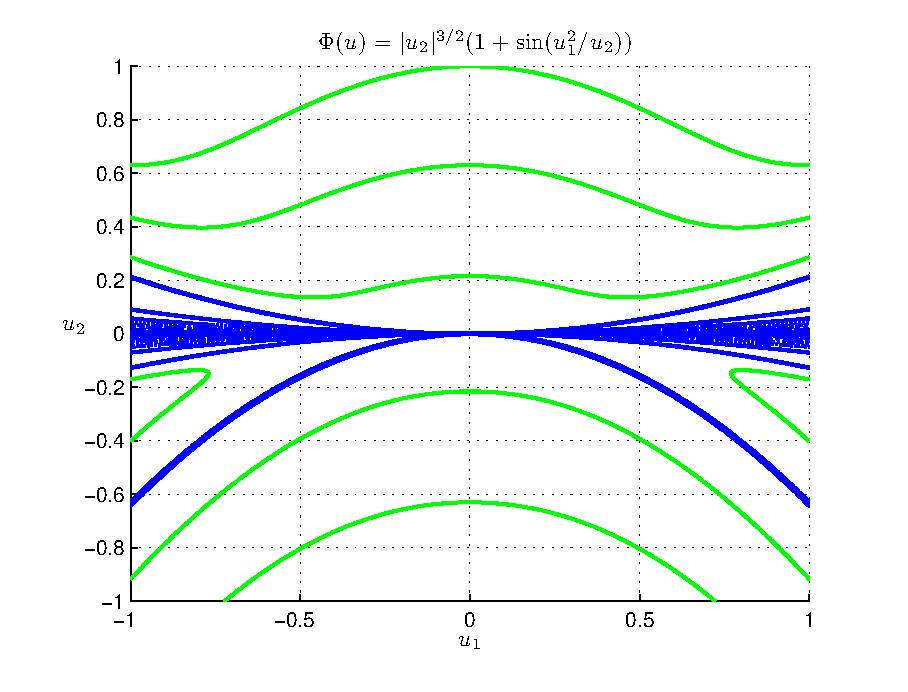
\includegraphics[width=0.7\maxpicturewidth]{your_figure.eps}
%   \center{Fig.~1. Your caption.}
% \end{figure}

\begin{references_eng}
% Insert your list of references here. The order of items in the list must
% agree with the order of their appearance in the text of your thesis.
% Use the '\url' command for citing url-s: e.g., \url{http://http://www.mathopt.org/}.

\item % Reference No. 1
  Domansky~V. Repeated games with asymmetric information and random price fluctuations at finance markets // International Journal of Game Theory. 2007. V.~36, \No~2. P.~241--257.

\item
  Aumann R.J., Maschler M.B. Repeated Games with Incomplete Information. Cambridge, Massachusetts: The MIT Press, 1995.

\item % Reference No. 2
  Domansky~V.C., Kreps~V.L. Game Theoretic Bidding Model: Strategic Aspects of Price Formation at Stock Markets // The Journal of the New Economic Association. 2011. V.~11. P.~39--62.

\item
  Chatterjee~K., Samuelson W. Bargaining under incomplete information //
  Operations Research. 1983. V.~31, \No 5. P.~835--851.

\item
  P'yanykh~A.I. A Multistage Exchange Trading Model with Asymmetric Information and Elements of Bargaining // Moscow University Computational Mathematics and Cybernetics. 2016. V.~40, \No~1. P.~35--40.
% ...

\end{references_eng}

%%%%%%%%%%%%%%%%%%%%%%%%%%%%%%%%%%%%%%%%%%%%%%%%%%%%%%%

%%% Local Variables:
%%% mode: latex
%%% TeX-master: "main"
%%% End:
